% ----------------------------------------------------------------------
% Packages
% ----------------------------------------------------------------------
\usepackage[T1]{fontenc}
\usepackage{babel,booktabs,csquotes,lmodern,tikz,verbatim}
% ----------------------------------------------------------------------

\usetikzlibrary{shapes}

% ----------------------------------------------------------------------
% New commands for this document
% ----------------------------------------------------------------------
\newcommand*\BibTeX{BibTeX}
\newcommand*\cls[1]{\textsf{#1}}
\newcommand*\cs[1]{\texttt{\char`\\#1}}
\newcommand*\marg[1]{\texttt{\char`\{#1\char`\}}}
\newcommand*\meta[1]{\ensuremath{\langle}\emph{#1}\ensuremath{\rangle}}
\newcommand*\oarg[1]{\texttt{[#1]}}
\newcommand*\pkg[1]{\textsf{#1}}

\renewcommand*\LaTeX{LaTeX}
\renewcommand*\LaTeXe{LaTeX2e}
\renewcommand*\TeX{TeX}
% ----------------------------------------------------------------------

% ----------------------------------------------------------------------
% Meta-data
% ----------------------------------------------------------------------
\title{\LaTeX\ Training Course}
\subtitle{\enquote{Using \LaTeX\ to write a thesis}}
\date{26th August 2011}
\author{UK-TUG Volunteers}
% ----------------------------------------------------------------------

\begin{document}

\begin{frame}
  \titlepage
\end{frame}

\mode<article>{\maketitle}

\tutornote{Time: 10:30}

\begin{frame}{Acknowledgements}

  \begin{itemize}
    \item Volunteers:
      \begin{itemize}
        \item Jay Hammond
        \item Phil Molyneux
        \item Joseph Wright
      \end{itemize}
    \item UK TeX Users' Group
    \item University of East Anglia
    \item Nicola Talbot
  \end{itemize}
  
\end{frame}

\section{An overview of \LaTeX}

\begin{frame}{What is \LaTeX, and what is \TeX?}

  \begin{itemize}
    \item \TeX{} is a typesetting application;
    \item \TeX{} uses \emph{primitives} to determine how to put text
      on a page;
    \item For most practical purposes, we need a \emph{format} built 
      on top of \TeX, for example:
      \begin{itemize}
        \item Plain \TeX;
        \item \LaTeX;
        \item Con\TeX{}t;
      \end{itemize}
    \item You can think of \LaTeX{} as an interpreter between you and
      \TeX.
  \end{itemize}

\end{frame}

\begin{frame}{\TeX{} \enquote{engines}}

  \begin{block}{pdf\TeX}
    The standard binary program: we'll be using this today.
  \end{block}
  
  \begin{block}{Xe\TeX}
    A merger of \TeX{} with modern font technology with support
    for native Unicode input and bidirectional typesetting.
  \end{block}
  
  \begin{block}{Lua\TeX}
    Also a modern engine: integrates the Lua scripting into \TeX.
  \end{block}
  
\end{frame}

\begin{frame}{What do we need to use \LaTeX?}

  \begin{itemize}
    \item A \TeX{} distribution: \TeX{}Live (Windows, Mac, Linux) or
      MiK\TeX{} (Windows only);
    \item A text editor, \emph{e.g.}~Notepad, TextEdit, Emacs;
    \item A PDF viewer, for example Adobe Reader.
  \end{itemize}

  \pause
  
  Usually, we use a specialist editor
  \begin{itemize}
    \item Coloured syntax;
    \item Buttons or menus to run \LaTeX{}, \emph{etc.};
    \item Most include an integrated spell checker.
  \end{itemize}
\end{frame}

\begin{frame}{Workflow}

  \resizebox{\linewidth}{!}{%
    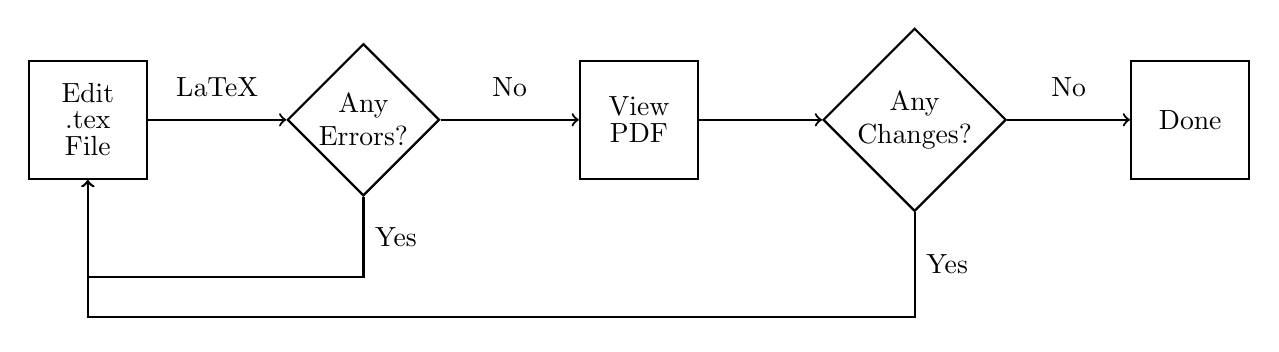
\begin{tikzpicture}[
      minimum width  = 1.5 cm,
      minimum height = 1.5 cm,
      inner sep      = 0.1 em,
      thick
    ]
      \path (0,0) node[draw] (edit) {\shortstack{Edit\\.tex\\File}} ;
      \path (3.5,0) node[draw,diamond] (errors) 
        {\shortstack{Any\\Errors?}};
      \path (7,0) node[draw] (pdf) {\shortstack{View\\PDF}};
      \path (10.5,0) node[draw,diamond] (change) 
        {\shortstack{Any\\Changes?}};
      \path (14,0) node[draw] (done) {Done};
      \draw[->] (edit) -- (errors) node[midway,above=-1em] 
        {\LaTeX};
      \draw[->] (errors) -- ++(0,-2) node[midway,right=-1em] 
        {Yes} -| (edit);
      \draw[->] (errors) -- (pdf) node[midway,above=-1em] {No};
      \draw[->] (pdf) -- (change);
      \draw[->] (change) -- ++(0,-2.5) node[midway,right=-1em] 
        {Yes} -| (edit);
      \draw[->] (change) -- (done) node[midway,above=-1em] {No};
    \end{tikzpicture}
  }
  
\end{frame}

\tutornote{10:45--11:15 Install \TeX}

\section{Getting started}

\begin{frame}{\LaTeX{} is not a word processor}

  \begin{itemize}
    \item \LaTeX{} input is stored as plain text files, usually with
      the extension \texttt{.tex};
    \item \LaTeX{} input files contain both the text of the document
      and \emph{control sequences};
    \item Control sequences start with a slash, so look like this:
      \cs{example}
    \item Writing in \LaTeX{} is therefore about \emph{programming}
      it to produce the document you want.
  \end{itemize}

\end{frame}

\begin{frame}{Spacing}

  \begin{itemize}
    \item \LaTeX{} treats multiple spaces as a single space;
    \item By default, the space between sentences is slightly larger
      than the space between words;
    \item This can be switched off using \cs{frenchspacing};
    \item New line characters are treated as a space;
    \item Paragraph breaks should be indicated by a blank line;
    \item \LaTeX{} automatically indents paragraphs, except for the
      first paragraph after a section heading.
  \end{itemize}
  
\end{frame}

\begin{frame}[fragile]{A simple document}
  \begin{example}
    \begin{semiverbatim}
\alert<2>{\\documentclass}\alert<2,4>{[a4paper,12pt]}\alert<2-3>{\{article\}}
\alert<5>{\% A comment in the preamble}
\alert<6>{\\begin\{document\}}
\alert<7>{\% This is a comment}
\alert<8>{This is   a simple}
\alert<8>{document\\footnote\{with a footnote\}.}

\alert<8>{This is a new paragraph.}
\alert<6>{\\end\{document\}}
    \end{semiverbatim}
  \end{example}
  
\end{frame}

\begin{exercise}
  Use the editor of your choice to create the above document. While you
  can use a specialist editor, start by doing this example in a basic
  editor such as Notepad. Save the document with a \texttt{.tex}
  extension, for example \texttt{exercise1.tex}, then go to a
  Terminal/Command Prompt and type:
  \begin{verbatim}
    pdflatex exercise1
  \end{verbatim}
  You can then view the resulting PDF file using a PDF viewer such as
  Adobe Reader.
\end{exercise}

\tutornote{Finish exercise at 11:45}

\section{Document Classes}

\begin{frame}{Document Classes}

  The \emph{document class} sets up the general layout of the document,
  for example:
   \begin{itemize}
     \item the format of the headings;
     \item if the document should have chapters;
     \item if the title should be on a separate page or above 
       the text on the first page.
   \end{itemize}

  \begin{block}{Usage}
      \cs{documentclass}\oarg{\meta{options}}\marg{\meta{class-name}}
  \end{block}
\end{frame}

\begin{frame}{Base classes}

  \begin{description}
    \item[\cls{article}] for short documents without chapters;
    \item[\cls{report}] for longer documents with chapters,
      typically single-sided with an abstract;
    \item[\cls{book}] for books, typically double-sided with
      front matter and back matter;
    \item[\cls{letter}] for correspondence;
    \item[\cls{slides}] for presentations.
  \end{description}

\end{frame}

\begin{frame}{Modern classes}

  \begin{description}
    \item[\cls{KOMA-Script}] \cls{scrartcl}, \cls{scrreprt}
      and \cls{scrbook} to replace \cls{article}, \cls{report}
      and \cls{book}, respectively;
    \item[\cls{memoir}] replaces \cls{book} and \cls{report};
    \item[\cls{beamer}] or slides (used to create the course 
      material).
  \end{description}
  
\end{frame}

\begin{frame}[fragile]{Documentation}

  \begin{block}{On your computer}
    The \texttt{texdoc} application will show documentation for 
    material you have installed. From the Command Prompt/Terminal
    \begin{center}
      \texttt{texdoc \meta{package}}
    \end{center}
  \end{block}
  
  \begin{block}{From CTAN}
    Try the web address
    \begin{center}
      \texttt{http://ctan.org/pkg/\meta{name}}
    \end{center}
  \end{block}

\end{frame}

\begin{frame}[fragile]{KOMA-Script Example}

  \verbatiminput{examples/example2}

\end{frame}

\begin{exercise}
  Try creating the above document. The KOMA-Script classes have
  various options that affect the document's appearance. Try
  experimenting with some of the following: \texttt{chapterprefix}, 
  \texttt{headings=small}, \texttt{headings=normal},
  \texttt{headings=big}, \texttt{numbers=enddot},
  \texttt{numbers=noenddot}.  For example:
  \begin{verbatim}
    \documentclass[chapterprefix]{scrreprt}
  \end{verbatim}
\end{exercise}

\tutornote{Finish exercise at 12:30 and go to lunch. Restart at
13:30.}

\section{Structure}

\begin{frame}{Title Page}

  First, you need to give the \enquote{meta-data}:
  \begin{itemize}
    \item \cs{title}\marg{\meta{title}}
    \item \cs{author}\marg{\meta{author(s)}}
    \item \cs{date}\marg{\meta{date}} (optional)
  \end{itemize}
   Then use \cs{maketitle} to display the title page.
   
   \vspace{2 em}
   
   \uncover<2>{%
     Classes such as KOMA-Script add more items, for example
     \cs{publisher}.%
   }

\end{frame}

\begin{frame}{Sectioning commands}

  Article-like classes provide the commands:
  \begin{itemize}
    \item \cs{part}\oarg{\meta{short title}}\marg{\meta{title}}
    \item \cs{section}\oarg{\meta{short title}}\marg{\meta{title}}
    \item \cs{subsection}\oarg{\meta{short title}}\marg{\meta{title}}
    \item \cs{subsubsection}\oarg{\meta{short title}}\marg{\meta{title}}
    \item 
      \alert<3>{\cs{paragraph}\oarg{\meta{short title}}\marg{\meta{title}}}
    \item \cs{subparagraph}\oarg{\meta{short title}}\marg{\meta{title}}
  \end{itemize}
  
  \vspace{2 em}
  \uncover<2->{%
     Book and report-like classes also provide the command:\\
    \cs{chapter}\oarg{\meta{short title}}\marg{\meta{title}}%
  }

\end{frame}

\begin{exercise}
  Try producing the following document.
  \verbatiminput{examples/example3}

  Here are some more KOMA-Script class options to try: 
  \texttt{appendixprefix}, \texttt{toc=flat}, \texttt{headsepline},
  \texttt{footsepline}.
\end{exercise}

\tutornote{Finish exercise at 14:30.}

\section{Graphics}

\begin{frame}{On packages}

  The \LaTeX{} kernel is rather limited: to get around that we
  load \emph{packages}:
  \begin{center}
    \cs{usepackage}\oarg{options}\marg{package}
  \end{center}
  or
  \begin{center}
    \cs{usepackage}\texttt{\{\meta{package1},\meta{package2},\ldots\}}
  \end{center} 
  We have already seen the \pkg{lipsum} package! 
  
  \vspace{1 em}
  
  \uncover<2>{%
   Documentation for packages is available in exactly the same way
   as for classes.%
  }
  
\end{frame}

\begin{frame}[fragile]{Including external images}

  \begin{itemize}
    \item Load the \pkg{graphicx} package to include graphics;
    \item Use \cs{includegraphics} to actually place the image;
    \item Image formats: \texttt{pdf}, \texttt{png}, \texttt{jpg};
    \item File extension should be omitted.
  \end{itemize}
  
  \vspace{1 em}
  \uncover<2>{%
    Graphics can also be \enquote{drawn} in \LaTeX{} using the
    Ti\emph{k}z package: a course in itself!
  }

\end{frame}

\begin{frame}[fragile]{Floating figures}

  \begin{block}{A basic figure}
\begin{semiverbatim}
\\begin\{figure\}\alert<2>{[htbp]}
\alert<3>{\\centering}
\\includegraphics\{myimage\}
\alert<4>{\\caption\{A Sample Figure\}}
\\end\{figure\}
\end{semiverbatim}
  \end{block}

\end{frame}

\begin{exercise}
  Try producing the following document. (Use an image application,
  such as paint, to produce a simple picture and save it as
  \texttt{shapes.png}.)
  \verbatiminput{examples/example4}
  Here are some more class options to try that will affect the list of
  figures: \texttt{chapteratlists}, \texttt{chapteratlists=0mm}.
\end{exercise}

\tutornote{Finish exercise at 15:00.}

\section{Bibliographies}

\begin{frame}{Creating a bibliography}

  \begin{itemize}
    \item Entries are stored in a \emph{\BibTeX{} database};
    \item Inform \LaTeX{} about it using \cs{bibliography} command;
    \item These are cited using \cs{cite} in the \LaTeX{} file;
    \item Choose a style using \cs{bibliographystyle}.
  \end{itemize}
  
\end{frame}

\begin{frame}[fragile]{Creating a bibliography}{The \LaTeX{} basics}

\begin{verbatim}
\documentclass{article}
\usepackage{natbib}
\bibliographystyle{plainnat}
\begin{document}
Some text \cite{key}.
\bibliography{example}
\end{document}
\end{verbatim}
  
\end{frame}

\begin{frame}{\BibTeX{} workflow}

  \small\mode<article>{\footnotesize}
  \resizebox{\linewidth}{!}{%
    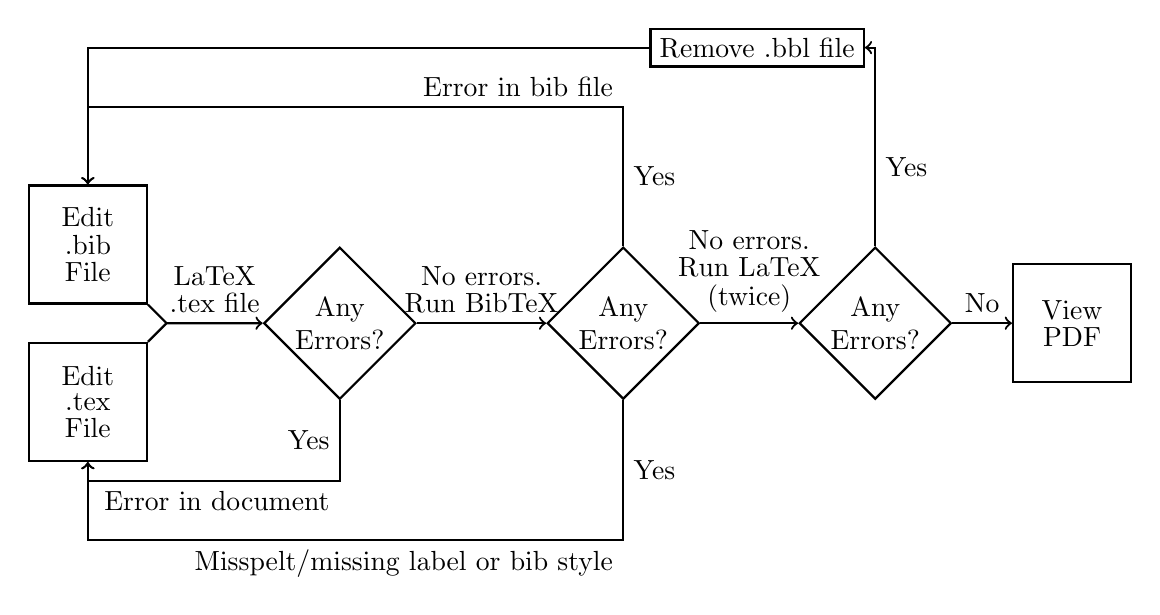
\begin{tikzpicture}[thick]
      \begin{scope}[minimum width=1.5cm,minimum height=1.5cm,inner sep=.1em]
        \path (0,0) node[draw] (edit) {\shortstack{Edit\\.tex\\File}};
        \path (0,2) node[draw] (editbib) {\shortstack{Edit\\.bib\\File}};
        \path (3.2,1) node[draw,diamond] (errors) 
          {\shortstack{Any\\Errors?}};
        \path (6.8,1) node[draw,diamond] (bibtexerrors)
          {\shortstack{Any\\Errors?}};
        \path (10,1) node[draw,diamond] (errors2)
          {\shortstack{Any\\Errors?}};
        \path (12.5,1) node[draw] (pdf) {\shortstack{View\\PDF}};
      \end{scope}
      \path (8.5,4.5) node[draw,rectangle] (rmbbl) {Remove .bbl file};
      \draw[->] (edit) -- (1,1) -- (errors) node[midway,above] 
        {\shortstack{\LaTeX\\.tex file}};
      \draw (editbib) -- (1,1);
      \draw[->] (errors) -- ++(0,-2) node[midway,left] {Yes}
        -| (edit) node[pos=0,below,anchor=north east] 
          {Error in document};
      \draw[->] (errors) -- (bibtexerrors)
        node[midway,above] {\shortstack{No errors.\\Run \BibTeX}};
      \draw[->] (bibtexerrors) -- ++(0,-2.75)
        node[midway,right] {Yes} -| (edit) 
        node[pos=0,below,anchor=north east] 
          {Misspelt/missing label or bib style};
      \draw[->] (bibtexerrors) -- ++(0,2.75) node[midway,right] 
        {Yes} -| (editbib) node[pos=0,above,anchor=south east] 
        {Error in bib file};
      \draw[->] (bibtexerrors) -- (errors2) node[midway,above] 
        {\shortstack{No errors.\\Run \LaTeX\\(twice)}};
      \draw[->] (errors2) |- (rmbbl) node[pos=0.2,right] {Yes};
      \draw[->] (rmbbl) -| (editbib);
      \draw[->] (errors2) -- (pdf) node[midway,above] {No};
    \end{tikzpicture}%
  }

\end{frame}

\begin{frame}[fragile]{The \BibTeX{} file}{A basic article}

  \begin{example}
    \begin{semiverbatim}
\alert<2>{@article}\{\alert<3>{lamport94},
   author    = "Leslie Lamport",
   title     = 
     "\alert<4>{\{\\LaTeX\}}: a document preparation system",
   edition   = "2nd",
   publisher = "Addison-{}-Wesley",
   year      = \alert<5>{1994},
\}
    \end{semiverbatim}
  \end{example}

\end{frame}

\begin{frame}[fragile]{The \BibTeX{} file}{Multiple authors}

  \begin{example}
    \begin{semiverbatim}
@inproceedings\{smith05,
  author    = "Smith, Jr, John \alert<2>{and} Jane Lucy Doe
   \alert<2>{and} and Other, Andrew N. \alert<2>{and} de Vere, Jo",
  title     = "An example article",
  booktitle = "Proceedings of the Imaginary Society",
  month     = JAN
  year      = 2005
\}
    \end{semiverbatim}
  \end{example}

\end{frame}

\begin{frame}[fragile]{Citations in \LaTeX}

  \begin{itemize}
    \item The \LaTeX{} kernel is limited for citations;
    \item The \pkg{natbib} package is much more powerful;
    \item A new approach is provided by \pkg{biblatex}.
  \end{itemize}

\end{frame}

\begin{frame}{Citations using \pkg{natbib}}

  \begin{block}{Textual citations}
    \vspace*{0.5 em}
    \begin{tabular}{l@{\ $\Rightarrow$\ }l}
      \multicolumn{2}{l}{%
        \cs{citet}\oarg{\meta{note}}\marg{\meta{key}}%
      } \\[0.5em]
      \cs{citet}\marg{lamport1994} & Lamport (1994) \\
      \cs{citet}\oarg{p.\textasciitilde34}\marg{lamport1994} &
        Lamport (1994, p.~34) \\
    \end{tabular}
  \end{block}
  
  \begin{block}{Parenthetical citations}
    \vspace*{0.5 em}
    \begin{tabular}{l@{\ $\Rightarrow$\ }l}
      \multicolumn{2}{l}{%
        \cs{citep}\oarg{\meta{prenote}}\oarg{\meta{postnote}}%
        \marg{\meta{key}}%
      }  \\[0.5em]
      \cs{citep}\marg{lamport94} & (Lamport, 1994)\\
      \cs{citep}\oarg{p.\textasciitilde34}\marg{lamport94} 
        & (Lamport, 1994, p.~34)\\
      \cs{citep}\oarg{see}\oarg{}\marg{lamport94} & (see Lamport, 1994)
    \end{tabular}
  \end{block}
  
\end{frame}

\begin{exercise}
  Create a file called \texttt{myrefs.bib} that contains the
  following:
  \verbatiminput{examples/myrefs.bib}

  Then create a file called, say, \texttt{example5.tex} that contains
  the following:
  \verbatiminput{examples/example5.tex}

  If you are using a terminal or command prompt, you will need to use
  the following commands:
  \begin{verbatim}
    pdflatex example5
    bibtex example5
    pdflatex example5
    pdflatex example5
  \end{verbatim}

  There are various options you can pass to the \pkg{natbib} package
  that affects the formatting. For example:
  \begin{verbatim}
    \usepackage[numbers,sort&compress]{natbib}
  \end{verbatim}
  Try experimenting with some of these options: \texttt{round},
  \texttt{curly} and \texttt{numbers}. With the \texttt{numbers}
  option, you can also use: \texttt{super}, \texttt{sort}
  and \texttt{sort\&compress}.
\end{exercise}

\tutornote{Finish exercise at 15:30 and have refreshments. Q\&A
session starts at 16:00.}

\section{Further information}

\begin{frame}{Getting help}

  \begin{itemize}
    \item \url{www.tex.ac.uk/faq};
    \item \url{wwww.latex-community.org};
    \item \url{tex.stackexchange.com};
    \item \url{theoval.cmp.uea.ac.uk/~nlct/latex/}.
  \end{itemize}

\end{frame}

\begin{frame}{Reading}

  \begin{itemize}
    \item \emph{Not So Short Introduction to \LaTeXe}, Oetiker;
    \item \emph{A Guide to \LaTeX}, Kopka and Daly;
    \item \emph{\LaTeX{} Beginners Guide}, Kottwitz.
  \end{itemize}

\end{frame}

\end{document}

